\section{Introduction}
Let $\Omega \subset \mathbb{R}^n$ represent a sufficiently smooth manifold and $V$ an infinite dimensional Hilbert space. Suppose we wish to solve the following linear boundary value problem: find $u \in V$ such that
\begin{align}
	B(v, u) = L(w)	\quad \forall v \in V \label{eq:1}
\end{align}
We will be interested in problems where the bilinear operator $B(\cdot,\cdot)$ features multi-scale behavior. These problems are typically difficult to solve with standard numerical methods. 

Lets take a variational multi-scale approach to make the multi-scale behavior apparent. Consider the following scale decomposition,
\begin{align}
	&V = \overline{V} \oplus V'&    &\text{with } &       & \mathcal{P} (u') = 0  \quad \forall u' \in V'&
\end{align}
Here $\overline{V}$ is typically finite dimensional and $V'$ is infinite dimensional. Furthermore, $\mathcal{P} \: : \; V \mapsto \overline{V}$ is the projector that defines the scale separation.

With this scale decomposition we can rewrite (\ref{eq:1}) as follows: find $\overline{u} \in \overline{V}$ and $u' \in V'$ such that
\begin{align}
	 B(\overline{v}, \overline{u}) + B(\overline{v}, u')  &= L(\overline{v})	\quad \forall \overline{v} \in \overline{V} \label{eq:2} \\
	 B(v', \overline{u}) + B(v', u')  &= L(v')	     \quad \forall v' \in V' \label{eq:3}
\end{align}
Here (\ref{eq:2})  is called the coarse scale equation and (\ref{eq:3}) the fine scale equation. Note that no simplifications have been made so far. The coarse and fine scale equations together are completely analogues to (\ref{eq:1}). The multi-scale behavior becomes apparent though if we rewrite the fine scale equation as follows,
\begin{align*}
	B(v', u')  &= L(v') - B(v', \overline{u}) 	     \quad \forall v' \in V'
\end{align*}
Here we can observe that the fine scales are driven by the residual of the coarse scales. Ultimately we would like to somehow incorporate the effect of the fine scales in the coarse scale equation and obtain a good discrete approximation $\overline{u}$ with our coarse scale space. Typically, the fine scale equation (\ref{eq:3}) is solved in an approximate way and its expression substituted into the coarse scale equation  (\ref{eq:2}) using static condensation.

We take a different approach and completely disregard the fine-scale equation, as experience has taught us that this equation is very hard to approximate well. To do so, we write the coarse scale equation in a different way as a Petrov Galerkin scheme: find $\overline{u} \in \overline{V}$ such that,
\begin{align}
	B(\overline{w}, \overline{u}) = L(\overline{w})	\quad \forall \overline{w} \in \overline{W} \label{eq:4}
\end{align}
where $\overline{W} \subset V$ is another finite dimensional Hilbert space. By requiring equality between (\ref{eq:2}) and (\ref{eq:4}) we can determine a test-space that will yield an optimal approximation $\overline{u}$ to $u$ in a norm of choice defined though the projector $\mathcal{P}$.

\subsection{Computing an optimal test-space}
We assume a basis for the finite dimensional Hilbert spaces $\overline{V}$ and $\overline{W}$ which is of the following form,
\begin{align}
	& \overline{V} := \mathrm{span} \left\{ \bar{\phi}_i(x), \; i=0,1,...,n   \right\} & &\text{and} &
	& \overline{W} := \mathrm{span} \left\{ \bar{\phi}_i(x) +  \psi_i'(x), \; i=0,1,...,n   \right\} &
\end{align}
Furthermore, we assume that $\bar{\phi}_i(x)$ and $\psi_i'(x)$, $i=0,1,...,n$ have equal compact support. The set of functions $\left\{ \psi_i', \; i=0,1,...,n  \right\}$ still remains unknown up to this point.  We will solve a local adjoint problem subject to the chosen projector $\mathcal{P}$ in order to determine each $\psi_i'$. The result is that the coarse scale solution $\overline{u} \in \overline{V}$ is the optimal solution to $u \in V$ in the norm defined through the projector.

The Petrov Galerkin scheme (\ref{eq:4}) is then equivalent to the following $n+1$ equations,
\begin{align}
	B(\overline{\phi}_i, \overline{u}) + B(\psi_i', \overline{u}) = L(\overline{\phi}_i) + L(\psi_i') 	\quad \text{for } i=0,1,...,n 
\end{align}
The coarse scale equation in the variational multi-scale decomposition, on the other hand, can be written as the $n+1$ equations,
\begin{align}
	B(\overline{\phi}_i, \overline{u}) + B(\overline{\phi}_i, u') = L(\overline{\phi}_i)  	\quad \text{for } i=0,1,...,n 
\end{align}
Equality between (\ref{eq:2}) and (\ref{eq:4}) implies equality of the above two equations for each $i=0,1,...,n$. So we have that,
\begin{align*}
	B(\overline{\phi}_i, u') &= B(\psi_i', \overline{u}) - L(\psi_i') \\
					 &= - B(\psi_i', u') 
\end{align*}
for each $i \in \left\{0,1,...,n\right\}$

So far we haven't made any assumptions on $\overline{\psi}_i $ other then them having compact support. It seems natural, however, to choose $\overline{\psi}_i \in V'$. This leads to the following Galerkin problem: find $\psi_i' \in V'$ such that,
\begin{align}
	\begin{cases} B(\psi_i ' , u') &= - B(\overline{\phi}_i, u') \quad \text{in } \Omega_i \quad \forall u' \in V' \\
	\left. \psi_i' \right|_{\partial \Omega_i} &= 0
	\end{cases}
	\label{eq:9}
\end{align} 
with $\Omega_i:=\mathrm{supp} \left(  \phi_i \right)$. This is a well posed problem given that the original global problem is well posed.
\begin{remark}
	At first glance this is a fine scale equation which seems equally hard to solve as the fine scale equation in the variational multi-scale decomposition. However, a more careful look reveals the following: 
	\begin{enumerate}
		\item Homogeneous boundary conditions.
		\item For each $i=0,1,...,n$ the equation is local; defined on the the domain $\Omega_i:=\mathrm{supp} \left(  \phi_i \right) \subset \Omega$.
	\end{enumerate}
	Both these points are a direct consequence of using compactly supported basis functions.
\end{remark}

Analytically solving (\ref{eq:9}) may still prove infeasible in the general setting. However, a sub-grid discretization based on an enriched space can lead to an excellent numerical approximation of $\psi_i' \in V'$. Here we show preliminary results where such a testspace is numerically computed using an enriched space


\subsection{Application to univariate advection diffusion problems}
Consider $\Omega = [0,1] $ and let $u,v \in H^1(\Omega)$. We introduce the following symmetric and asymmetric  bilinear forms,
\begin{align}
	& a(u,v) =  \left( \nabla v, \nabla u   \right)_{\Omega}, &
	& b(u,v) = -\left( \nabla v, Pe \cdot u   \right)_{\Omega} & 
\end{align}
where $Pe \in \mathbb{R}$ denotes the Peclet number.

The continuous problem is as follows:
\begin{align}
\begin{cases} & \text{given $l \in H^{-1}$, find $u \in H^1(\Omega)$ such that: } \\
	& a(u,v) + b(u,v) = l(v) \quad \forall v \in H^1_0(\Omega)  \\
	& u(0) = g_0, \; u(1) = g_1  
\end{cases}
	\label{eq:cd1}
\end{align}

Numerically solving (\ref{eq:cd1}) starts by choosing the proper finite dimensional subspaces for the trial and test variables. Let $\left\{ \phi_i, \; i=0,1,2,...,n \right\}$ be a basis for piece-wice $C^0$ polynomials with minimum compact support. Following the introduction we define the two finite dimensional Hilbert spaces,
\begin{align}
	&  \overline{V} := \mathrm{span} \left\{ \bar{\phi}_i(x) \in H^1(\Omega), \; i=0,1,...,n   \right\} & \\
	&  \overline{W} := \mathrm{span} \left\{ \bar{\phi}_i(x) +  \psi_i'(x) \in H^1(\Omega), \; i=0,1,...,n   \right\} &
\end{align}
where we assume that $\phi_i \in \overline{V}$ and $\psi_i \in V'$ have equal compact support. $\left\{ \psi_i', \; i=0,1,2,...,n \right\}$ is still unknown and follows from the solution of $n+1$ local adjoint problems (\ref{eq:9}). Let the support of $\bar{\phi}_i(x)$ be [a,b]. Then we have the following constraint saddle-point problem for each $\psi_i'$, $i=0,1,...,n$, 
\begin{align}
\begin{cases} & \text{given $\bar{\phi}_i \in H^{1}(\Omega)$, find $\psi_i' \in V' \subset H^1_0 (\Omega)$ and $\bar{\lambda} \in \overline \subset H^1_0 (\Omega)$ such that: } \\
	& a(u',\psi_i') + b(u',\psi_i') + (\mathcal{P} u', \bar{\lambda}) = a(u',\bar{\phi}_i) + b(u', \bar{\phi}_i)  \quad \forall u' \in V' \subset H^1_0(0,1)  \\
	& \text{subject to: } \\
	& (\bar{u}, \mathcal{P} \psi_i') = 0 \quad \forall \bar{u} \in \overline{V} \subset H^1(\Omega) \\
	& \bar{\psi}'_i(a) = \psi_i'(b) = 0  
\end{cases}
		\label{eq:testfun}
\end{align}
This is a well posed problem, by virtue of (\ref{eq:cd1}) being well posed. The particular form of the solution  $\left\{ \psi_i', \; i=0,1,2,...,n \right\}$ depends on the chosen projector $\mathcal{P}$ that provides the scale separation $H^1(\Omega) = \overline{V} \oplus V'$. In the following we choose the $H^1_0$-semi-norm to provide scale separation. The corresponding projector, denoted   $\mathcal{P} \; : \: H^1(0,1) \mapsto \overline{V}$ is defined through the following problem: find $\overline{u} \in \overline{V}$ such that for all $\overline{v} \in \overline{V}$,
\begin{align}
	& a(\overline{v}, \overline{u}) = a(\overline{v}, u) &  
	&  \Longleftrightarrow &
	& a(\overline{v}, u - \overline{u}) = 0  &
	&  \Longleftrightarrow &
	& a(\overline{v}, u') = 0 &
\end{align}

After the test functions have been determined by solving (\ref{eq:testfun}), either analytically or numerically, we can proceed and solve the global coarse scale problem by means of the proposed Petrov Galerkin scheme: with $l \in H^{-1}$, find $\overline{u} \in  \overline{V} \subset H^1(0,1)$, such that
\begin{align}
\begin{cases} & \text{given $l \in H^{-1}$, find $\bar{u} \in \overline{V} \subset H^1(\Omega)$ such that: } \\
	& a(\bar{u},\bar{v}) + b(\bar{u},\bar{v}) = l(\bar{v}) \quad \forall \bar{v} \in \overline{W} \subset H^1_0(\Omega)  \\
	& \bar{u}(0) = g_0, \; \bar{u}(1) = g_1  
\end{cases}
	\label{eq:cd2}
\end{align}

\begin{remark} (\ref{eq:cd2})  is equivalent to the discrete set of equations $\vect{K}{} \vect{u}{} = \vect{f}{}$, where,
\begin{align}
	& \vect{K}{ij} = a(\bar{\phi}_i, \bar{\phi}_j) + a(\psi_i', \bar{\phi}_j)  + b(\bar{\phi}_i, \bar{\phi}_j) + b(\psi_i', \bar{\phi}_j) &
	&\text{and }&
	& \vect{f}{i} = l(\bar{\phi}_i) + l(\psi_i')   &
\end{align}
for $i,j = 0,1,2,...,n-1$, subject to the given Dirichlet data.
\end{remark}

\begin{remark} $a(\psi_i', \bar{\phi}_j)$  is trivially zero due to the $H^1_0(\Omega)$ semi-norm projector $\mathcal{P}$. This also implies that the proposed Petrov Galerkin scheme reduces to standard Galerkin in the case of a pure diffusion problem.
\end{remark}

\begin{remark} $b(\psi_i', \bar{\phi}_j)$  is positive definite and symmetric. I still need to prove this. Hence, this is the term that provides the stability.
\end{remark}

Below follow some initial results using linear and quadratic finite elements. Figures \ref{fig:optimaltestfunc1} and \ref{fig:optimaltestfunc2} illustrate the computation of the optimal test functions for a two element partition. Figure \ref{fig:optimaltestfunc3} computes the numerical solution using this same basis for an advection diffusion problem with $Pe = 10$. Finally Figures \ref{fig:optimaltestfunc4} and \ref{fig:optimaltestfunc5} compute the numerical solution on a ten element partition to an advection diffusion problem with $Pe = 500$ and homogeneous and non-homogeneous right-hand-side, respectively. 
\begin{figure}
	\centering
	\subfigure[$p = 1$]{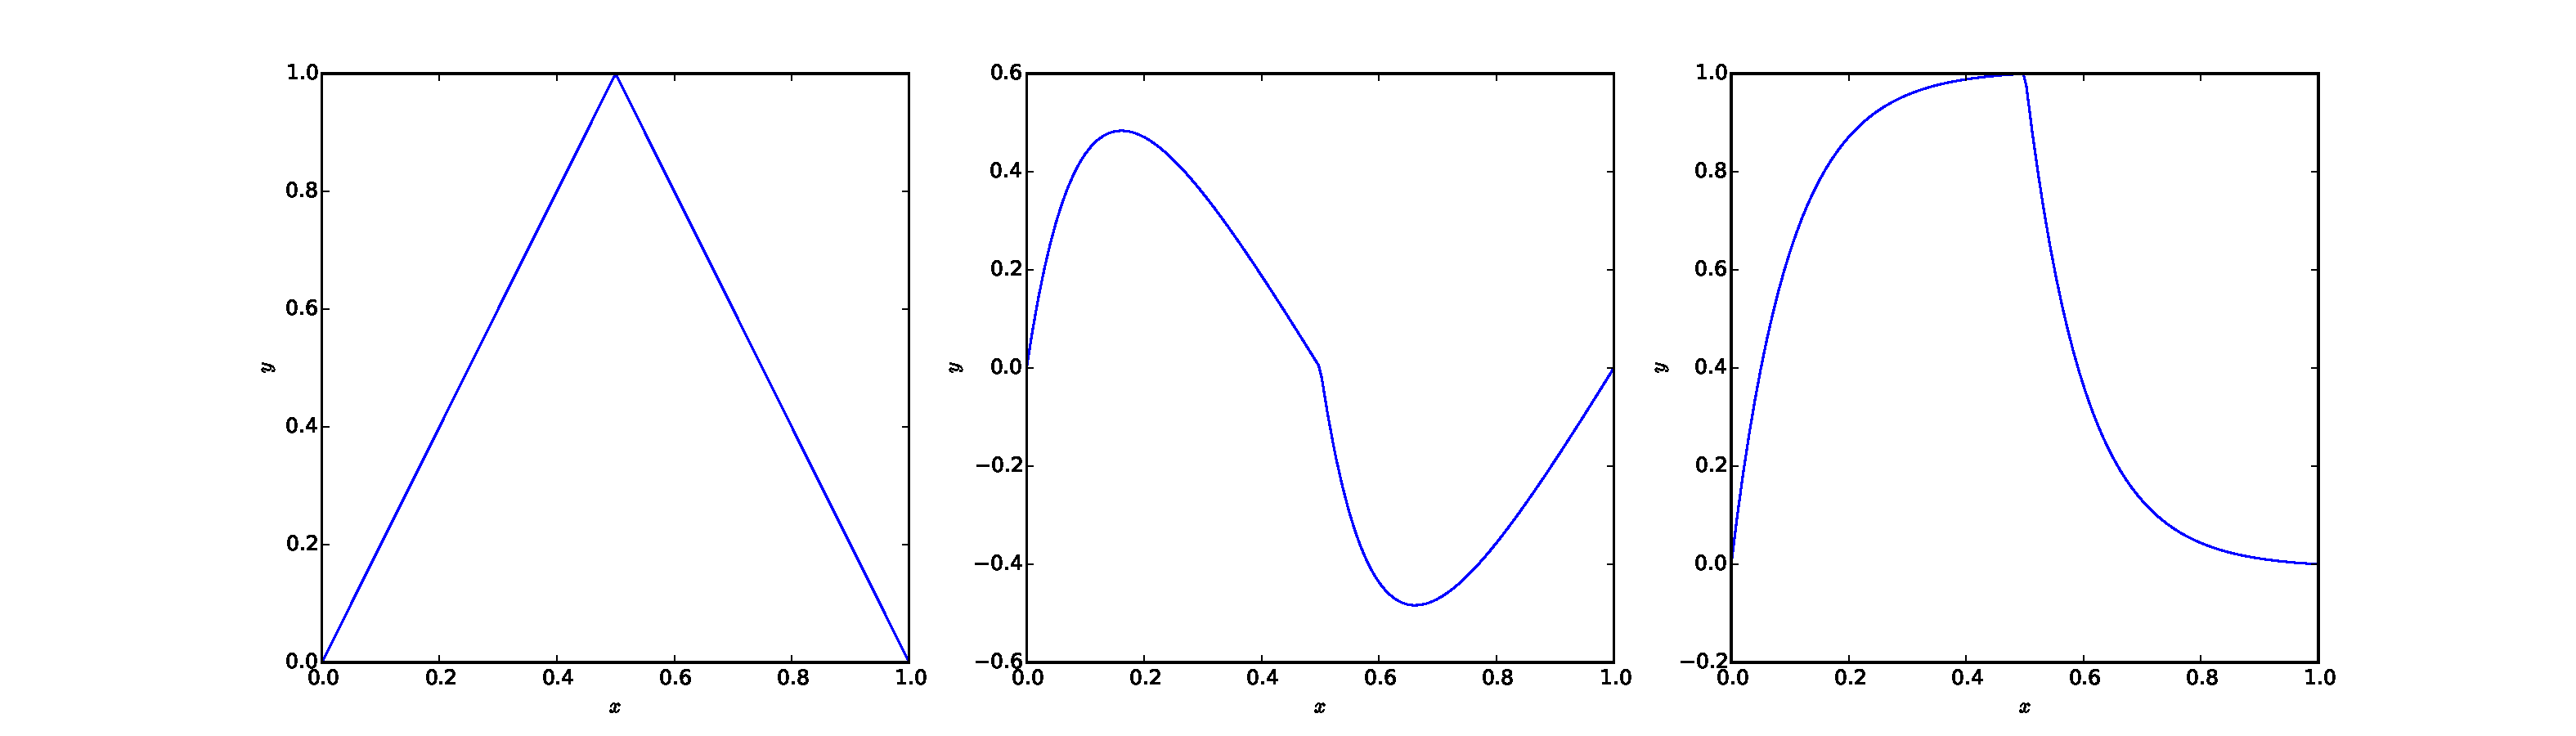
\includegraphics[trim = 0cm  0cm 0cm 0cm,clip,width=1\textwidth]{figures/optimaltestfunction_degree_1_Peclet_10}} \\
	\subfigure[$p = 2$]{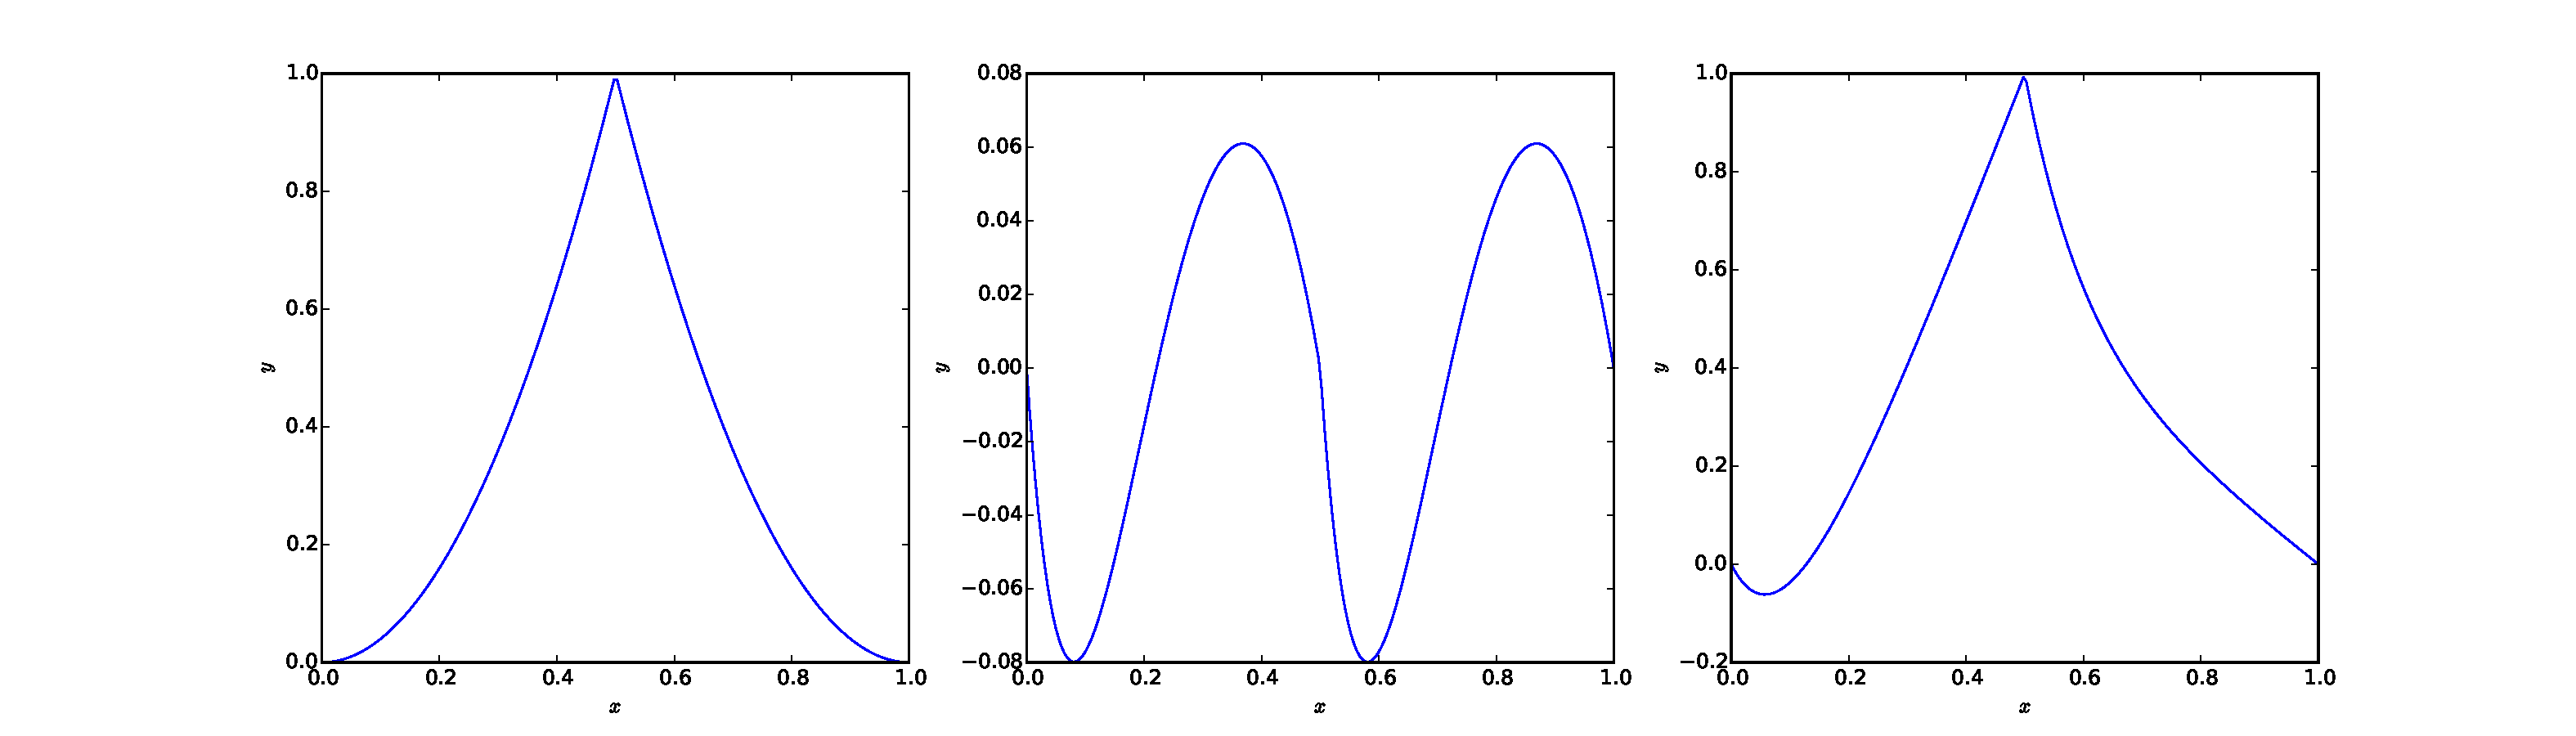
\includegraphics[trim = 0cm  0cm 0cm 0cm,clip,width=1\textwidth]{figures/optimaltestfunction_degree_2_Peclet_10}} 
	\caption{Calculation of optimal test-functions in the $H^1_0$ semi-norm for linear and quadratic finite elements at $Pe=10$. (Left) Coarse scale function $\bar{\phi}_i$. (Middle)  fine scale part $\psi_i'$. (Right) optimal test-function as the sum of the coarse scale function and a fine scale part $\bar{\phi}_i + \psi_i'$.}
	\label{fig:optimaltestfunc1}
\end{figure}

\begin{figure}
	\centering
	\subfigure[$p = 1$]{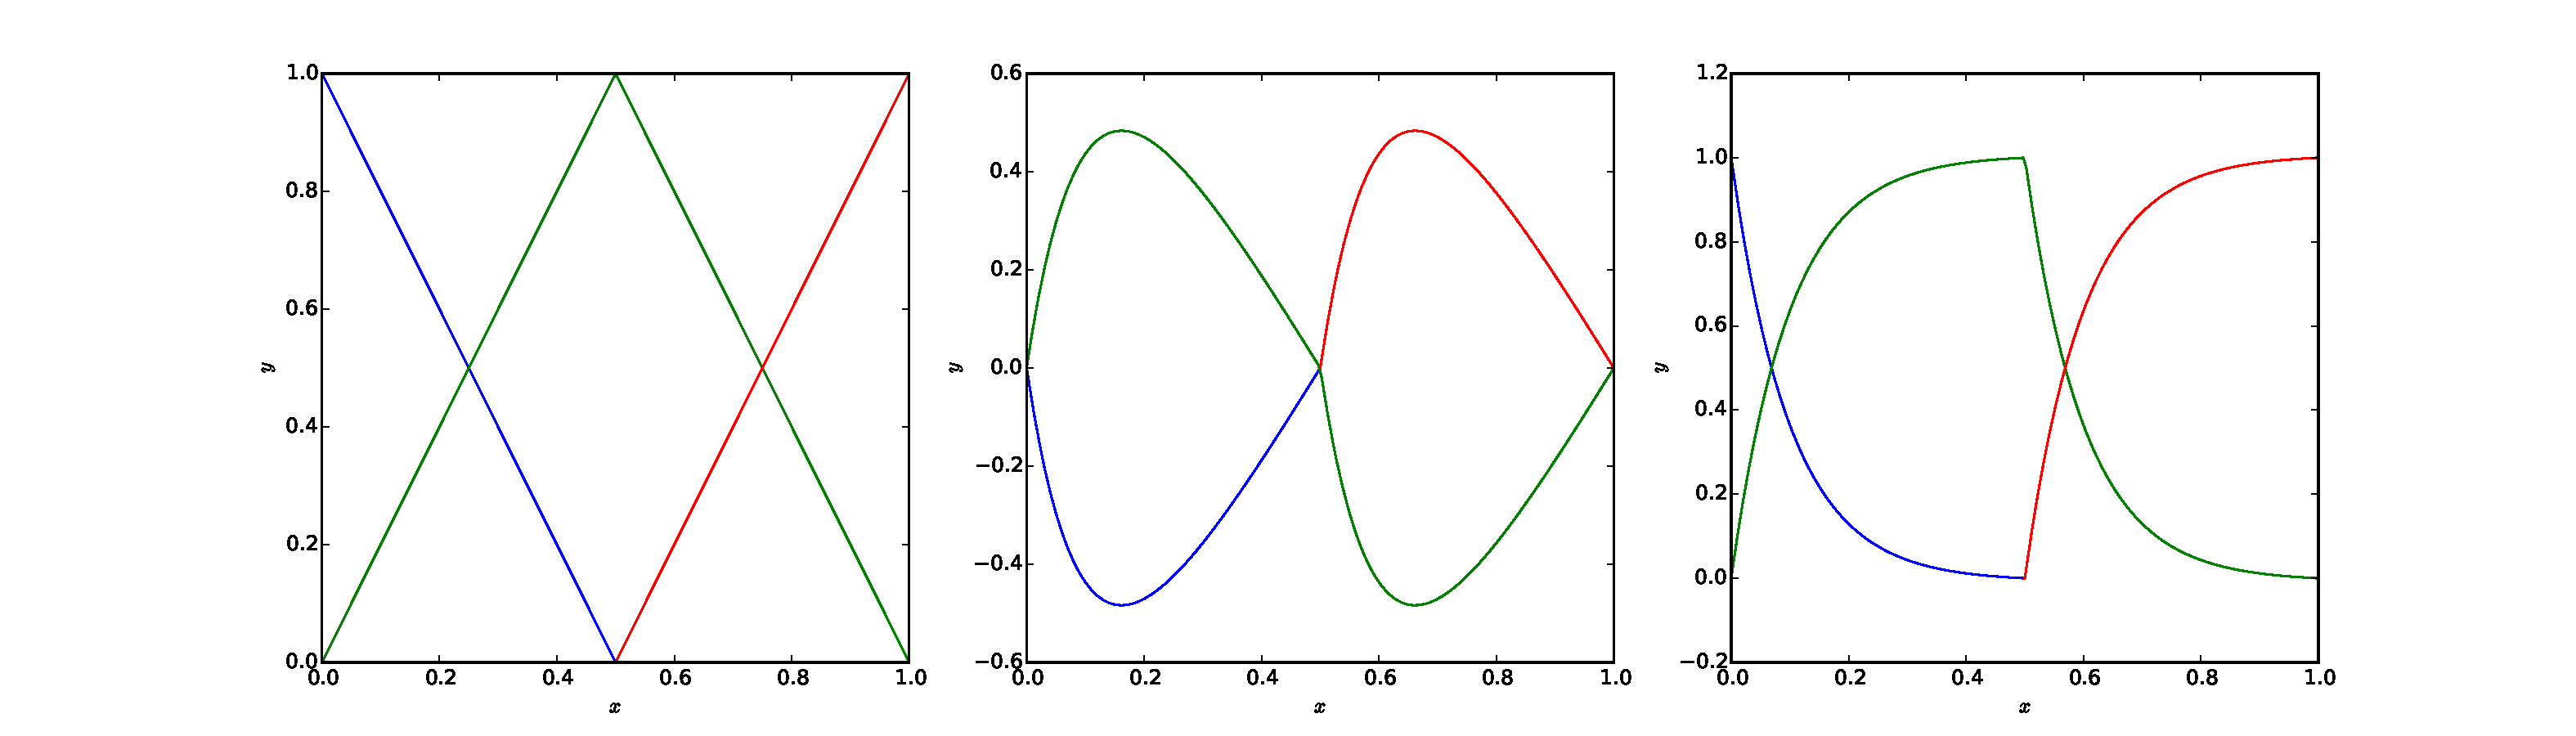
\includegraphics[trim = 0cm  0cm 0cm 0cm,clip,width=1\textwidth]{figures/optimaltestbasis_degree_1_Peclet_10}} \\
	\subfigure[$p = 2$]{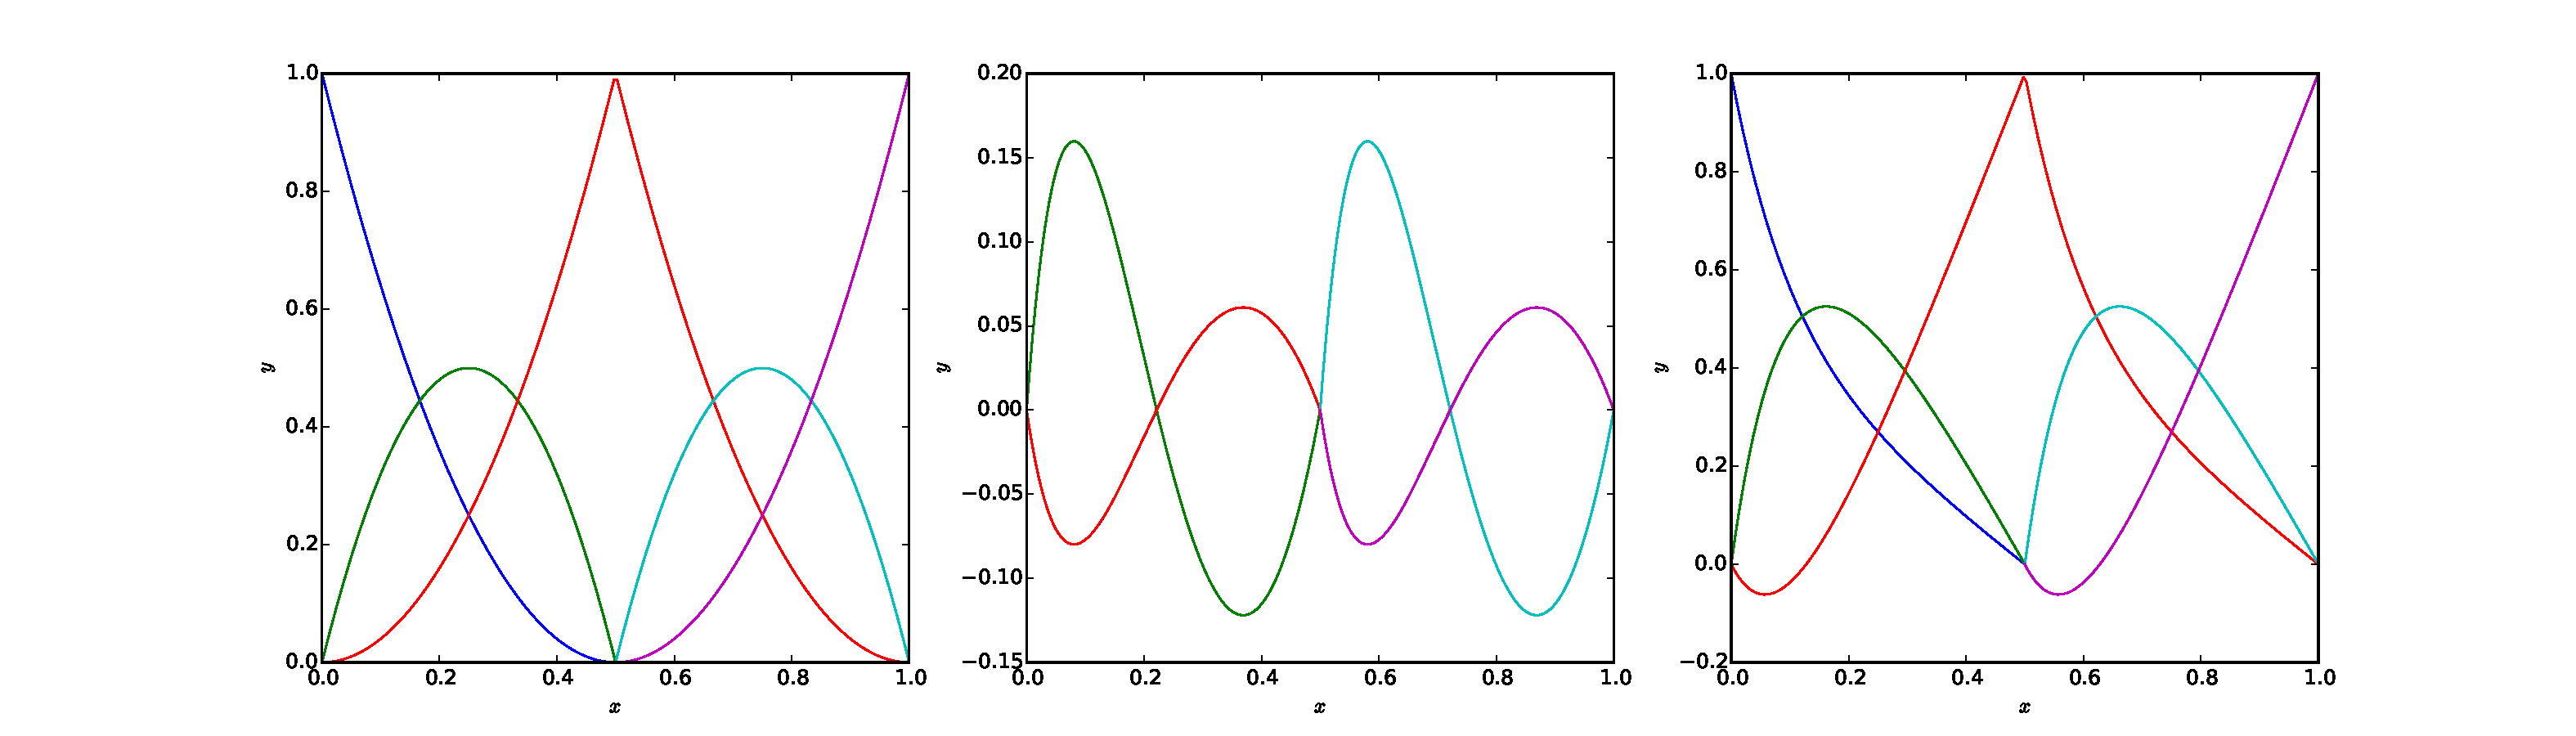
\includegraphics[trim = 0cm  0cm 0cm 0cm,clip,width=1\textwidth]{figures/optimaltestbasis_degree_2_Peclet_10}} 
	\caption{Optimal basis in the $H^1_0$ semi-norm for the test-space for linear and quadratic finite elements at $Pe=10$. (Left) Basis for the coarse scales. (Middle)  part due to the fine scale behaviour. (Right) optimal basis as the sum of the coarse scale function and a fine scale part.}
	\label{fig:optimaltestfunc2}
\end{figure}

\begin{figure}
	\centering
	\subfigure[$p = 1$]{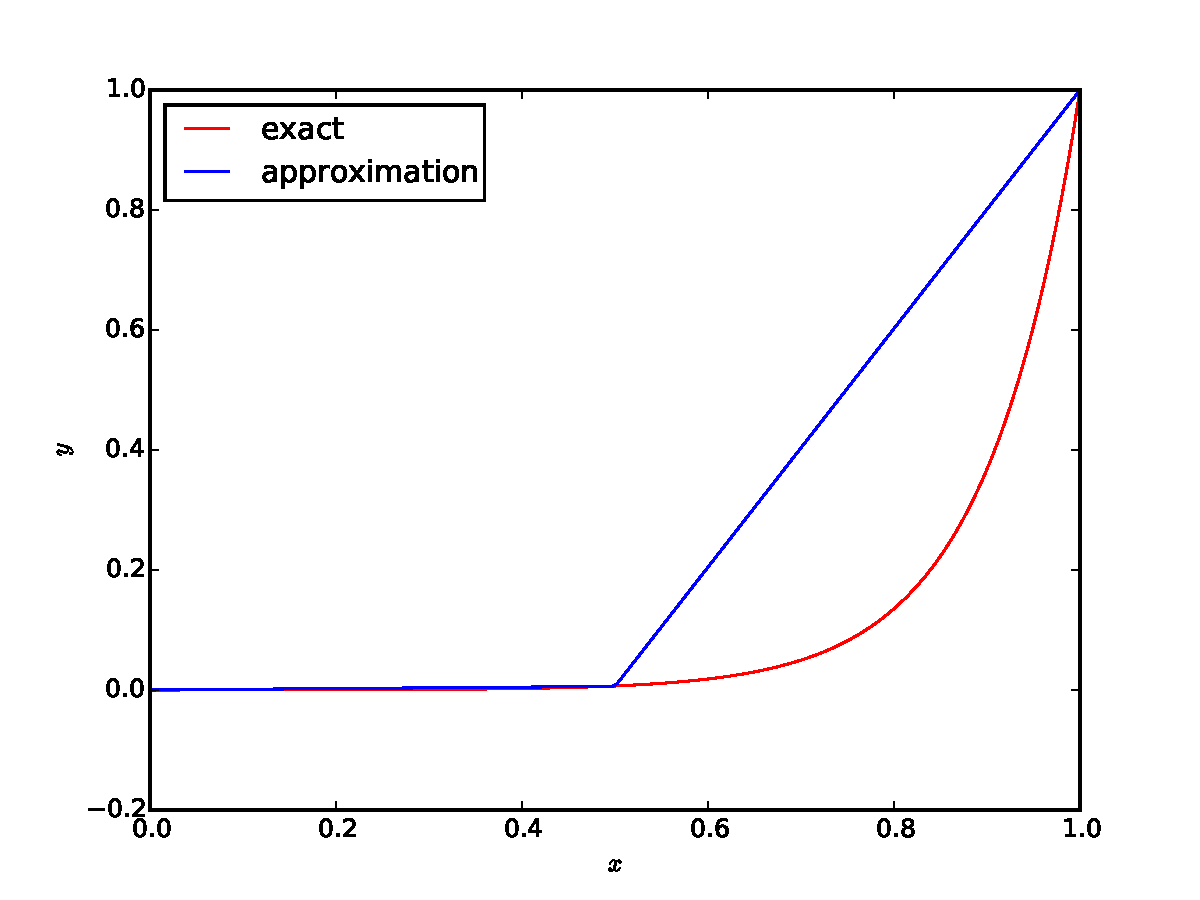
\includegraphics[trim = 0cm  0cm 0cm 0cm,clip,width=0.49\textwidth]{figures/optimalsolution_degree_1_Peclet_10}}
	\subfigure[$p = 2$]{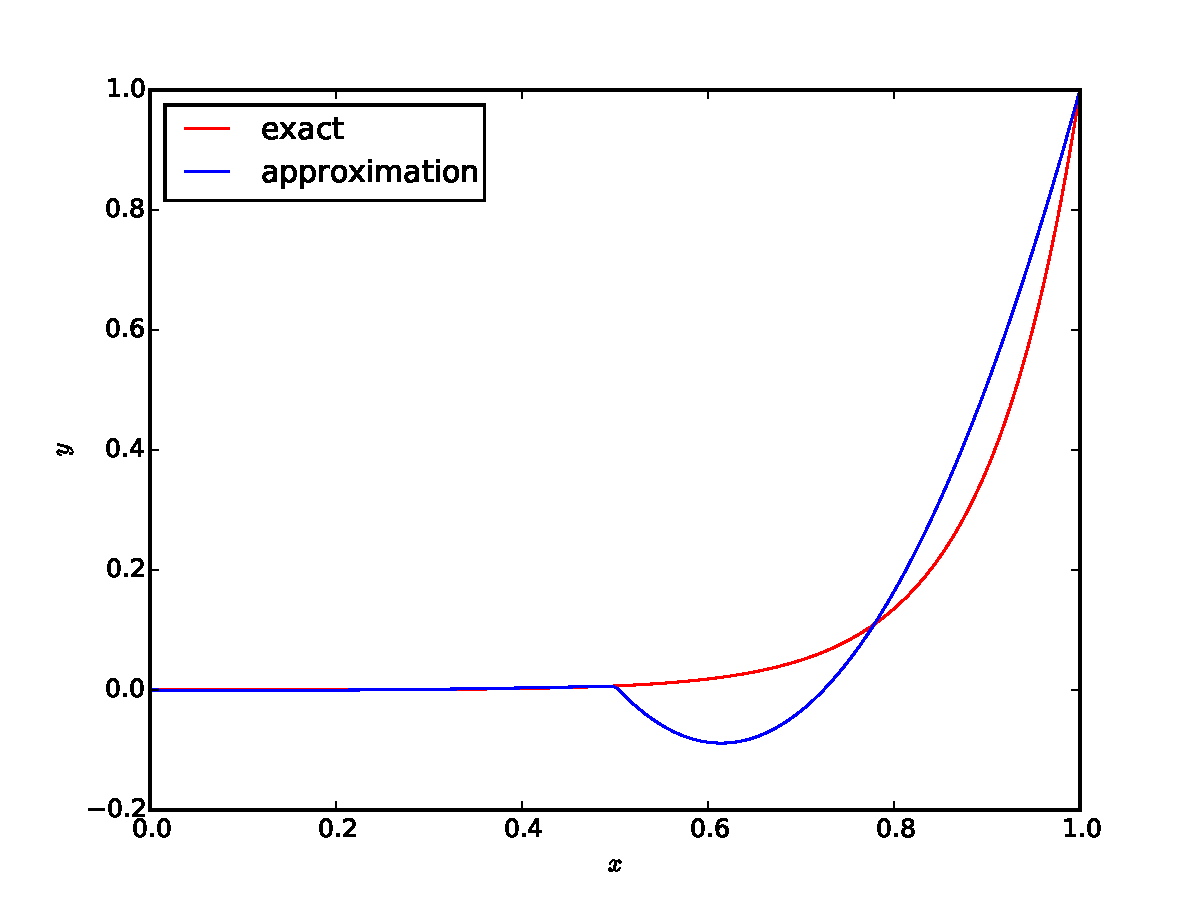
\includegraphics[trim = 0cm  0cm 0cm 0cm,clip,width=0.49\textwidth]{figures/optimalsolution_degree_2_Peclet_10}} 
	\caption{Optimal numerical solution in the $H^1_0$ semi-norm obtained using linear and quadratic continuous Petrov Galerkin with optimal testing on a partition of 2 elements.}
	\label{fig:optimaltestfunc3}
\end{figure}


\begin{figure}
	\centering
	\subfigure[$p = 1$]{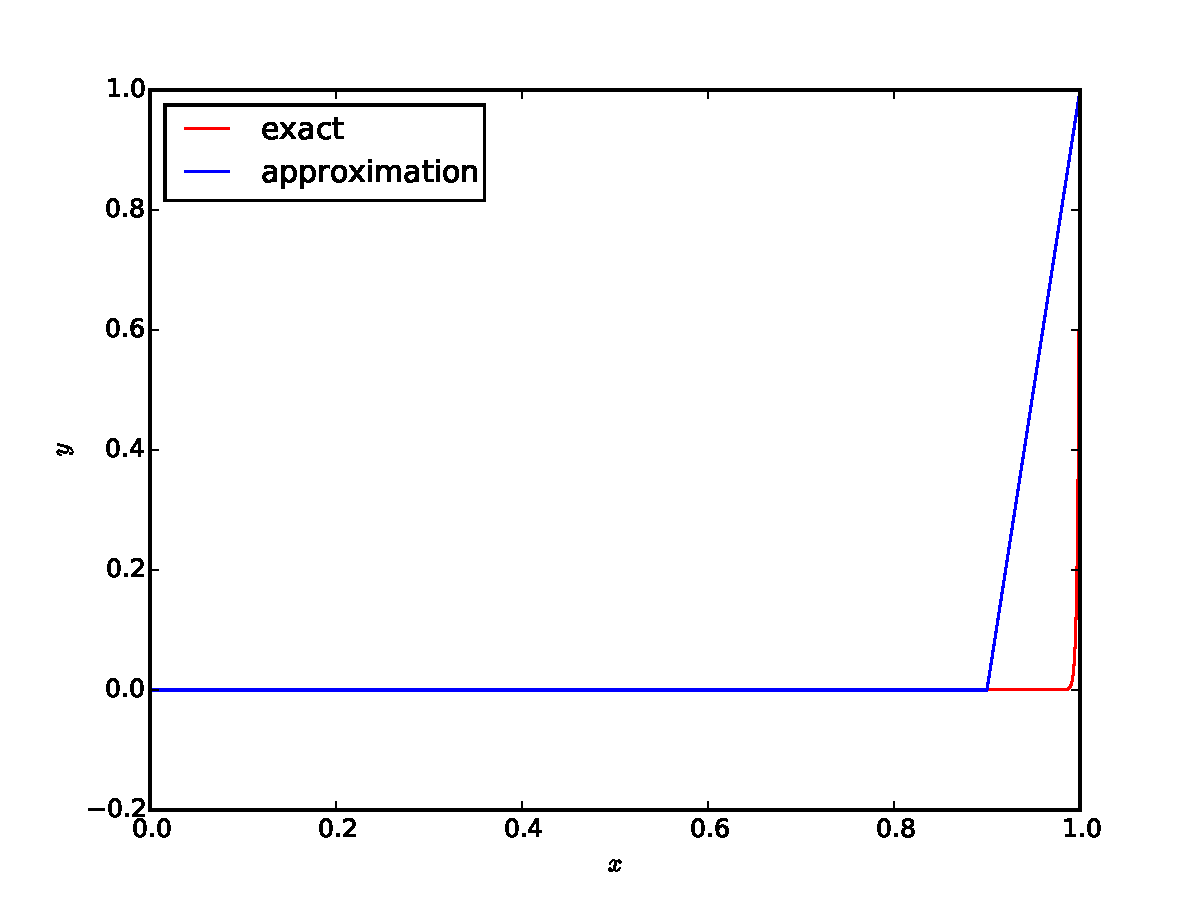
\includegraphics[trim = 0cm  0cm 0cm 0cm,clip,width=0.49\textwidth]{figures/optimalsolution_degree_1_Peclet_500_1}}
	\subfigure[$p = 2$]{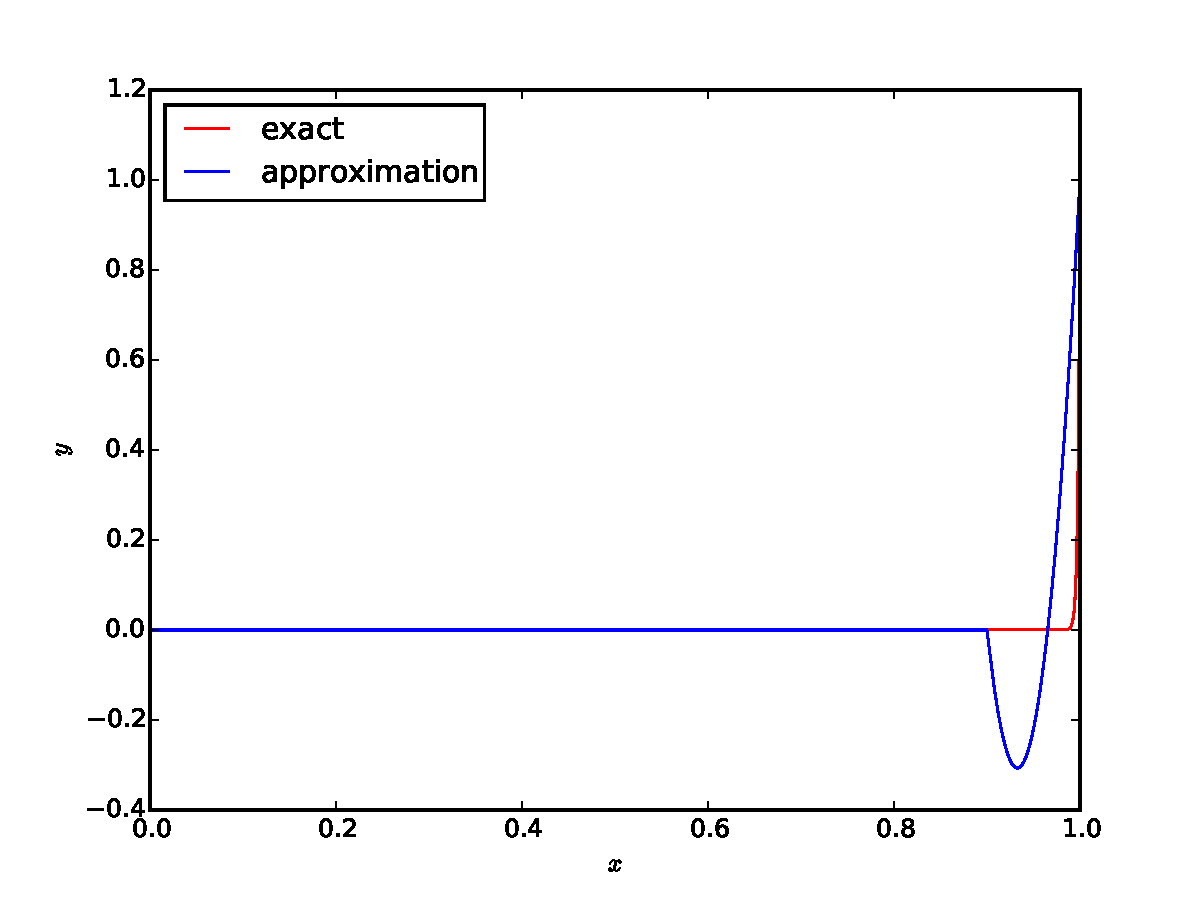
\includegraphics[trim = 0cm  0cm 0cm 0cm,clip,width=0.49\textwidth]{figures/optimalsolution_degree_2_Peclet_500_1}} 
	\caption{Test problem 1 with a zero right hand side and $Pe =500$. Optimal numerical solution in the $H^1_0$ semi-norm obtained using linear and quadratic continuous Petrov Galerkin with optimal testing  on a partition of 10 elements}
	\label{fig:optimaltestfunc4}
\end{figure}

\begin{figure}
	\centering
	\subfigure[$p = 1$]{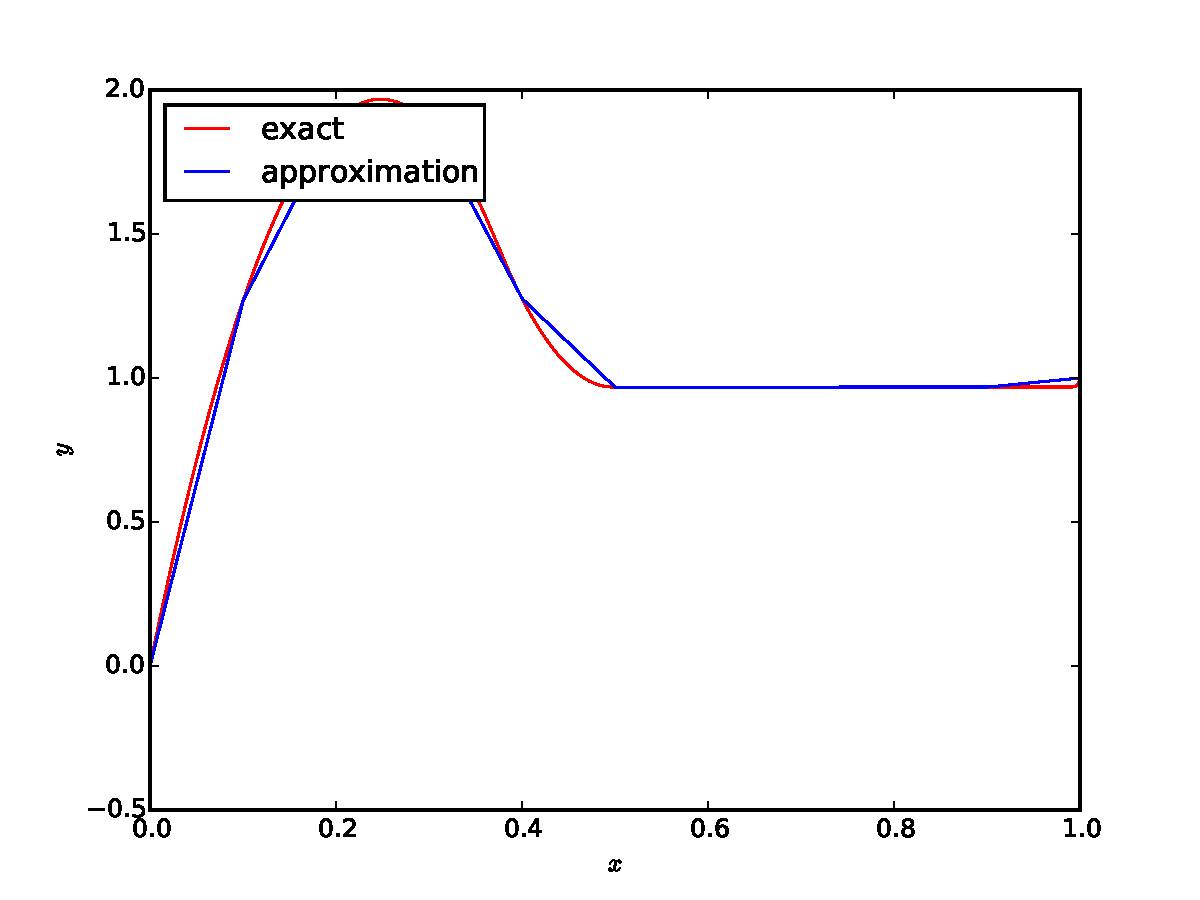
\includegraphics[trim = 0cm  0cm 0cm 0cm,clip,width=0.49\textwidth]{figures/optimalsolution_degree_1_Peclet_500_2}}
	\subfigure[$p = 2$]{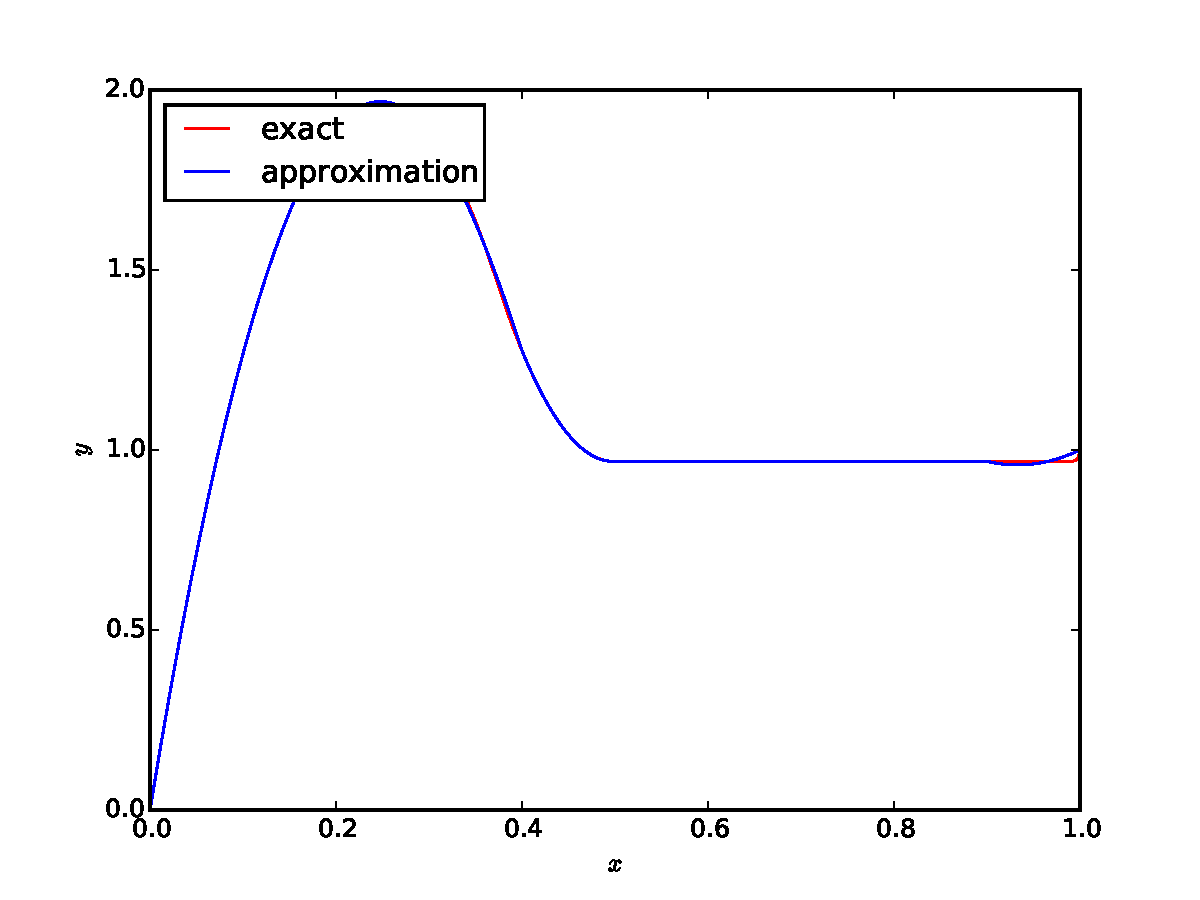
\includegraphics[trim = 0cm  0cm 0cm 0cm,clip,width=0.49\textwidth]{figures/optimalsolution_degree_2_Peclet_500_2}} 
	\caption{Test problem 2 with a non-zero right-hand-side and $Pe=500$. Optimal numerical solution in the $H^1_0$ semi-norm obtained using linear and quadratic continuous Petrov Galerkin with optimal testing  on a partition of 10 elements.}
	\label{fig:optimaltestfunc5}
\end{figure}





















